\documentclass[12pt]{article}
\usepackage[utf8]{inputenc}
\usepackage[T1]{fontenc}
\usepackage[french]{babel}
\usepackage[top=2.5cm]{geometry}
\usepackage{graphicx}
\usepackage{caption}
\usepackage{subcaption}
\usepackage{chemfig}
\usepackage{amsmath}
\usepackage{amssymb}
\usepackage{amsfonts}
\usepackage{csquotes}
\usepackage{url}

\newcommand{\equ}{\Longleftrightarrow{}}
\newcommand{\deriv}{\mathrm{d}}
\newcommand{\dt}[1]{\frac{\deriv #1}{\deriv t}}
\newcommand{\dtau}[1]{\frac{\deriv #1}{\deriv \tau}}


\title{Projet dynamique des populations cellulaires :\\
``NONLINEAR DYNAMICS OF IMMUNOGENIC TUMORS: PARAMETER ESTIMATION AND GLOBAL BIFURCATION ANALYSIS''}
\author{Célestin \bsc{Bigarré}}
\date{Février 2020}

\begin{document}

\maketitle
\section*{Introduction}
Ce projet étudie le modèle proposé par Kuznetsov dans son article ``\emph{Nonlinear  Dynamics of Immunogenic Tumors: Estimation and global Bifurcation Analysis}'' de 1994. Ce modèle décrit les intéraction entre une tumeur cancéreuse et le système immunitaire et cherche à décrire les dynamiques de la maladie ainsi que les effets du système immunitaire sur la régulation de la population cancéreuse. 

\paragraph{} En particulier, les auteurs cherchent à reproduire les effets de ``dormance tumorale'' qui correspond au fait pour une tumeur de petite taille de rester dans un état quiescient avec un très faible taux de croissance mais une résistance accrue aux traitement et à la réponse immunitaire (amenant à la rechute de maladie apparement guérie jusqu'à plusieurs dizains d'années après la fin du traitement).

Un autre effet que le modèle cherche à expliquer est le phénomène de ``sneaking through'' defini par Klein \cite{klein_1966} comme \textquote{the preferential take of tumours after small size inocula to a similar degree with that seen with large size inocula, compared to the rejection of medium sized inocula}. C'est-à-dire comme le fait pour une tumeur de petite taille, de s'implanter avec une grande probabilité (comparable à celle d'une tumeur de très grande taille) alors que les tumeur de taille moyenne ont une plus faible probabilité de s'implanter. Les méchanismes de ``sneaking through'' permettent donc aux très petite tumeurs d'échapper au système immunitaire jusqu'à ce qu'elle aient atteint une taille critique quin'est plus régulable par l'organisme. 

\paragraph{}Pour obtenir ces résultats les auteurs proposent un modèle méchaniste qui prend en compte les effets d'immunostimulation, c'est-à-dire les effets positifs du système immunitaire sur la croissance tumorale dans certaines conditions. Il arrive en effet que la stimulation du système immunitaire, au lieu de freiner la croissance tumorale, ait au contraire un effet d'accélération de cette croissance. 

\section{Modèle}
\subsection{modèle complet}
Les auteurs cherchent à modéliser les interactions entre une tumeur et le système immunitaire. Il partent donc de de deux populations de cellules, les cellules tumorales (T) et les cellules effectrices du système immunitaire (E). Il écrivent leur modèle à partir du schéma de réaction de la Figure \ref{fig:reaction}. 

L'interaction entre les cellules T et E forme avec un taux $k_1$, des complexes C. Ces complexes peuvent se dissocier sans dommages (avec un taux $k_{-1}$). Les complexes peuvent aussi se dissocier en entraînant la programation de la mort de la cellule tumorale (avec un taux $k_2$) ou l'inactivation définitive de la cellule effectrice (avec un taux $k_3$).
\begin{figure}[h]
    \centering
    \schemestart E + T\arrow{<=>[$k_1$][$k_{-1}$]} C \arrow(bb--.base west){->[$k_2$]}[45, 0.75] E + T* \arrow(@bb--.north west){->[][$k_3$]}[-45, 0.75]E* + T\schemestop\par
    \caption{Schéma de réaction entre la Tumeur et le système immunitaire. Repris de \cite{kuznetsov}}
    \label{fig:reaction}
\end{figure}

Les auteurs écrivent donc le modèle d'équations différentielles ordinaires suivant : 

\begin{align}
\dt{E} &= s + F(C, T) - d_1 E  k_1 ET + (k_{-1} + k_2) C\label{equ:dE/dt}\\
\dt{T} &= a T ( 1 - b T_{\mathrm{tot}} ) - k_1 E T + (k_{-1} - k_2) C\label{equ:dT/dt}\\
\dt{C} &= k_1 ET - (k_{-1} + k_2 + k_3) C\label{equ:dC/dt}\\
\dt{E*} &= k_3 C - d_2 E* \label{equ:dE*/dt}\\
\dt{T*} &= k_2 C - d_3 T*\label{equ:dT*/dt}
\end{align}
Où $T_{\mathrm{tot}} = T + C$ est la population totale de la tumeur. $s$ est le taux d'arrivée de cellules effectrices dans la tumeur au niveau basal (sans prendre en compte l'effet de la tumeur sur le système immunitaire). La fonction $F$ caractérise le taux d'accumulation des cellules effectrices dans la tumeur lié à la présence de celle-ci, par stimulation soit de leur migration, soit de leur multiplication. $d_1$, $d_2$ et $d_3$ sont les taux d'élimination (quelque soit la cause) respectivement des cellules E, E* et T*.


\subsection{Simplification du modèle}
On peut remarquer que les variables $E*$ et $T*$ n'interviennent pas dans les équations (\ref{equ:dE/dt}) (\ref{equ:dC/dt}) et (\ref{equ:dT/dt}). Comme les quantité qui nous intéressent sont $E$ et $T$. Nous pouvons oublier les équations (\ref{equ:dE*/dt}) et (\ref{equ:dT*/dt}) qui ne sont finalement pas utiles pour comprendre le comportement du système. 

\paragraph*{} De précédents travaux indiquent qu'une forme possible pour $F$ est : 
\begin{equation}
    F(C, T) = \frac{fC}{g + T}, \label{equ::F}
\end{equation}

avec $g>0$, $f>0$

\paragraph*{}Les échelles de temps différent de plusieurs ordres de grandeur entre les réactions mises en jeu. Le temps de formation des complexes entres cellules effectrices et cellules tumorales est de l'ordre de la dizaine de minutes alors que la multiplication de cellules effectrices prend une dizaine d'heure. On peut donc faire une approximation d'état quasi-statique, qui s'exprime par
\begin{align}
    \frac{\deriv C}{dt} &=0 \notag\\
    \Longrightarrow C&= KET \label{equ::C}\\
    \intertext{avec, }
    K &=\frac{k_1}{k_{-1} + k_2+k_3}\notag
\end{align}


\paragraph{}De plus, les cellules tumorales impliquées dans un complexe représentent une petite proportion de toutes les cellules tumorales. Cela nous conduit à l'approximation suivante, 
\begin{equation}
    \Longrightarrow T_{tot} \sim T \label{equ::Ttot}
\end{equation} 

\paragraph{}En regroupant \ref{equ:dE/dt}, \ref{equ:dT/dt}, \ref{equ::C}, \ref{equ::F} et \ref{equ::Ttot} on arrive au système simplifié portant uniquement sur les deux variables $E$ et $T$ :
\begin{equation}
    \left\{\begin{aligned}
    \frac{\deriv E}{\deriv t} &= s + \frac{pET}{g+ T} - mET -dE\\
    \frac{\deriv T}{\deriv t} &= a T \left(1-bT\right) - nET
    \end{aligned}\right.
    \label{equ::model}
\end{equation}
avec, 
\begin{equation*}
\begin{aligned}
    &p = fK\\
    &m = Kk_3\\
    &n = Kk_2\\
    &d = d_1
\end{aligned}
\end{equation*}

\subsection{Estimation des paramètres du modèle}
Pour estimer les paramètres du modèle, les auteurs se sont basés sur la littérature. Les estimations utilisées sont issues de d'expériences sur un modèle murin de Lymphôme B chronique. 

Les paramètres retenus sont les suivants : 
\begin{align*}
    a &= 0.18 \,\texttt{jour}^{-1}\\
    b &= 2.0 \times 10^{-9} \,\texttt{cellules}^{-1}\\
    s &= 1.3 \times 10^4 \,\texttt{cellules jour}^{-1}\\
    p &= 0.1245  \,\texttt{jour}^{-1}\\
    g &= 2.019 \times 10^7  \,\texttt{cellules}\\
    m &= 3.422 \times 10^{-10} \,\texttt{cellules}^{-1} \texttt{jour}^{-1}\\
    n &= 1.101 \times 10^{-7} \\
    d &= 0.0412 \,\texttt{jour}^{-1}\\
    E_0 &= 10^6 \,\texttt{cellules}\\
    T_0 &= 10^6 \,\texttt{cellules}\\
\end{align*}

\subsection{Adimensionnement du modèle}
Posons le changement de variable, 
\begin{equation*}
    \left\{
    \begin{aligned}
        \tau &= n T_0 t\\
        x &= \frac{E}{E_0}\\
        y &= \frac{T}{T_0}
    \end{aligned}
    \right.
\end{equation*}
Ainsi que le changement de paramètres suivant (les valeurs correspondantes sont donnés à la Table \ref{table::param_bio} : 
\begin{align*}
    &\sigma = \frac{s}{n E_0 T_0}     & \rho = \frac{p}{nT_0}&\\
    &\eta = \frac{g}{T_0}  &\mu = \frac{m}{n} = \frac{k_3}{k_2}&\\
    &\delta = \frac{d}{nT_0} &\beta = bT_0&\\
    & \alpha = \frac{a}{nT_0} & &
\end{align*}
\begin{table}[h]
    \centering
    \begin{tabular}{|c|c|}
    \hline
         Paramètre & Valeur \\
    \hline
        $T_0$, $E_0$ & $10^6$ \\
        $\sigma$ & $0.1181$\\
        $\rho$ & $	1.131$\\
        $\eta$ & $ 	20.19$\\
        $\mu$ & $0.00311$\\
        $\delta$ &$0.3743$ \\
        $\alpha$ & $1.636$\\
        $\beta$ & $2.0\times 10^{-3}$\\
    \hline
    \end{tabular}
    \caption{Paramètres biologiques estimés pour le modèle adimensionné}
    \label{table::param_bio}
\end{table}

\paragraph{}On exprime le modèle en fonction de ces nouvelles quantités. La règle de dérivation composée donne: 
\[
\dt{x}\left[\tau(t)\right] = \dt{x}\left[\tau(t)\right]\times \frac{1}{\dt{\tau}(t)}
\]
Or, 
\[
    \dt{\tau}(t) = n T_0 \text{ et }
    \dt{x} = \frac{1}{E_0}\dt{E}
\]

D'où en utilisant \ref{equ::model} on trouve, les fonctions étant prises en $\tau$ :
\begin{align}
    \dtau{x} &= \frac{1}{E_0nT_0}\left[s + \frac{pET}{g+T}-mET -dE\right]  \notag\\
    &= \frac{1}{E_0nT_0}\left[
    \sigma n T_0 E_0 + \frac{\rho n T_0 x E_0 y T_0}{\eta T_0 + y T_0} -\mu n x E_0 y T_0 -\delta n T_0 x E_0
    \right] \notag\\
    &= \sigma + \frac{\rho xy}{\eta+y}-\mu xy -\delta x 
    \label{equ::dx/dtau}
\end{align}

\paragraph{}De même, on trouve pour $y$:
\begin{align}
    \dtau{y}\left[\tau(t)\right] &= \frac{1}{\dt{\tau}(t)}\times \dt{y}\left(\tau(t)\right) \notag\\
    &= \frac{1}{T_0^2n} \left[aT\left(1-bT\right)-nET \right]\notag\\
    &= \frac{1}{nT_0^2}\left[\alpha n T_0^2 y \left(1 - \frac{\beta}{T_0}T_0y\right)\right] \notag\\
    &= \alpha y \left(1-\beta y \right) -\frac{E_0}{T_0}xy\notag\\
    \Longleftrightarrow{} \dtau{y} &= \alpha y \left(1-\beta y \right) -xy \label{equ::dy/dtau}
\end{align}
En supposant que $E_0$ = $T_0$ comme indiqué par l'estimation biologique des paramètres


\paragraph{}Finalement, on trouve le modèle adimensionné composé des équations \ref{equ::dx/dtau} et \ref{equ::dy/dtau}:
\begin{equation}
    \left\{
    \begin{aligned}
        \dtau{x} &= \sigma + \frac{\rho xy}{\eta+y}-\mu xy -\delta x \\
        \dtau{y} &= \alpha y \left(1-\beta y \right) -xy
    \end{aligned}
    \right. \label{equ::modele_adimensionne}
\end{equation}


\section{Équilibres}
\subsection{Isoclines nulles}
Les isoclines du modèles sont les courbes de l'espace de phase le long desquelles, $dx/dt =0$ ou $dy/dt = 0$. Les points d'équilibres du modèles sont donnés par les points d'intersection des isoclines de $x$ et $y$.

\paragraph{}L'isocline nulle pour $x$ est donnée par
\begin{align*}
    &\dt{x} =0 \\
    \equ &\sigma + \frac{\rho xy}{\eta+y}-\mu xy -\delta x =0\\
    \equ &x = \frac{\sigma}{\delta + \mu y - \frac{\rho y}{eta+y}}
\end{align*}

\paragraph{}L'isocline nulle pour $y$ est donnée par
\begin{align*}
    &\dt{y} =0 \\
    \equ &\alpha y \left(1-\beta y \right) -xy =0\\
    \equ &\left\{\begin{aligned}
        y&=0\\
       &\text{ou}\\
       x &= \alpha \left(1-\beta y\right)
    \end{aligned}\right.
\end{align*}


\begin{figure}[!ht]
    \centering
    \begin{subfigure}[b]{0.49\textwidth}
         \centering
         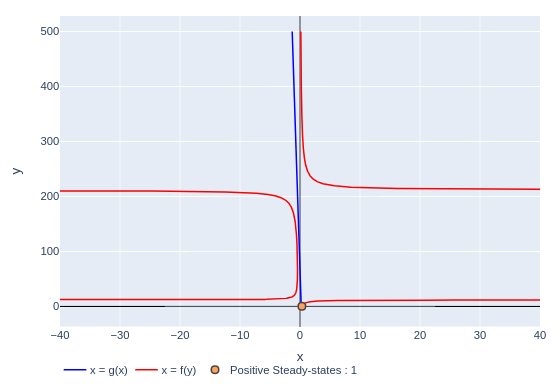
\includegraphics[width=\textwidth]{../figures/fig_isocline_2.png}
         \caption{$\beta = 0.015$, $\alpha=0.2$}
         \label{fig::nuclline 1 ss}
     \end{subfigure}
     \hfill
    \begin{subfigure}[b]{0.49\textwidth}
         \centering
         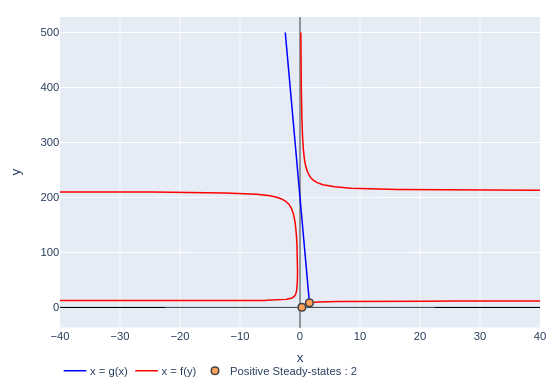
\includegraphics[width=\textwidth]{../figures/fig_isocline_1.png}
         \caption{$\beta = 0.005$, $\alpha=1.636$}
         \label{fig::nuclline 2 ss}
     \end{subfigure}\\
     \begin{subfigure}[b]{0.49\textwidth}
         \centering
         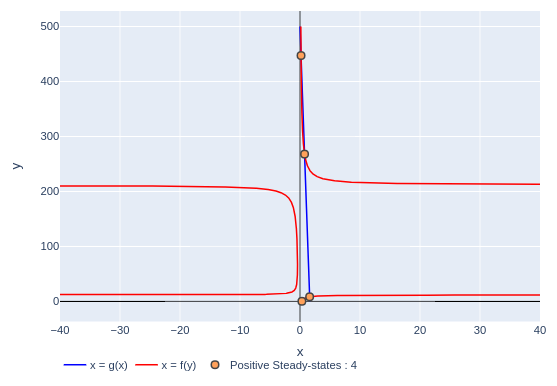
\includegraphics[width=\textwidth]{../figures/fig_isocline_0.png}
         \caption{$\beta = 0.002$, $\alpha=1.636$}
         \label{fig::nuclline 4 ss}
     \end{subfigure}
    \caption{Isoclines nulles et points d'intersections approximatifs pour différentes valeurs de paramètres. Les autres paramètres sont ceux du modèe biologique.}
    \label{fig:nullclines}
\end{figure}

\paragraph{}
On a tracé à la Figure \ref{fig:nullclines} les isoclines nulles du modèle pour différentes valeurs de $\beta$. On a représenté les points d'intersections graphiques des isoclines correspondants aux équilibres positifs. On arrive en faisant varier $\beta$ et $\alpha$ à obtenir $1$, $2$ ou $4$ équilibres positifs. 

\subsection{États d'équilibres}
Les points d'équilibres sont les solutions du système: 
\begin{equation*}
    \left\{
    \begin{aligned}
        \dt{x} &= 0\\
        \dt{y} &= 0,
    \end{aligned}\right.
\end{equation*}
c'est-à-dire les ponts d'intersections entre les isoclines de $x$ et de $y$. 

Le système se réécrit donc, 
\begin{align*}
    &\left\{
    \begin{aligned}
        x &= \frac{\sigma}{\delta + \mu y- \frac{\rho y}{\eta+ y }},  &y= 0\\
        x&=\alpha \left(1-\beta y\right),  &\frac{\sigma}{\delta + \mu y - \frac{\rho y}{\eta+y}} = \alpha \left(1-\beta y\right)
    \end{aligned}\right.\\
    \equ &\left\{
    \begin{aligned}
        x &= \frac{\sigma}{\delta}, &y = 0\\
        x&=\alpha \left(1-\beta y\right),  &\frac{\sigma (\eta+y)}{(\eta+y)(\delta + \mu y) - \rho y} = \alpha \left(1-\beta y\right)
    \end{aligned}\right.\\
    \intertext{On résout l'équation sur $y$ de la deuxième ligne,}
    \frac{\sigma (\eta+y)}{(\eta+y)(\delta + \mu y) - \rho y} &= \alpha \left(1-\beta y\right) &\equ\\
   \frac{\sigma}{\alpha} (\eta + y) &= (1 - \beta y) [\eta \delta + \eta \mu y + \delta y +\mu y^2 -\rho y] \\
   \begin{split}
   &=(1-\beta y) [\mu y^2 + (\eta\mu + \delta-\rho)y + \eta\delta]\\
   &= \mu y^2 +(\eta\mu+\delta -\rho)y+\eta\delta - \beta\mu y^3 + \beta(\rho - \delta-\eta\mu)y^2\\
   & \qquad-\beta\eta\delta y \end{split} &\equ\\
\begin{split}
0 &= -\beta\mu y^3 + (\mu +\beta(\rho-delta-\eta\mu))y^2\\ &\qquad+\left(\mu\eta+\delta-\rho-\beta\eta-\frac{\sigma}{\alpha}\right)y + \eta \left(\delta-\frac{\sigma}{\alpha}\right) 
\end{split} &\equ\\
\begin{split}
0 &= \beta\mu y^3 + (\beta(\delta+\eta\mu-\rho)- \mu)y^2 \\ &\qquad+\left(\rho+\beta\eta+\frac{\sigma}{\alpha}- \mu\eta - \delta \right)y
+ \eta \left(\frac{\sigma}{\alpha} - \delta\right) 
\end{split} 
\end{align*}
Les équilibres sont donc donnés par les solutions de:
\begin{align}
    & \left\{
    \begin{aligned}
        x &= \frac{\sigma}{\delta + \mu y- \frac{\rho y}{\eta+ y }}\\
        y &= 0
    \end{aligned}
    \right. \label{equ::equilibre_lin}\\
    \intertext{et de}
    & \left\{
    \begin{aligned}
        x &= \alpha (1 - \beta y)\\
        0 &= C_3 y^3 + C_2 y^2 +C_1 y + C_0
    \end{aligned}
    \right. \label{equ::equilibre_cubique}
    \intertext{avec}
    \begin{aligned}
        C_0 &= \eta \left(\frac{\sigma}{\alpha} - \delta\right) \\
        C_1 &= \rho+\beta\eta+\frac{\sigma}{\alpha}- \mu\eta - \delta \\
        C_2 &= \beta(\delta+\eta\mu-\rho)- \mu\\
        C_3 &= \beta\mu
    \end{aligned}\notag
\end{align}

\subsection{Détermination du nombre maximal d'équilibres}
On s'intéresse maintenant au nombre d'équilibres positifs du systèmes car ce sont ceux qui correspondent à des situations biologiques possibles. 

\paragraph{}
L'équation (\ref{equ::equilibre_lin}) admet une unique solution positive dès que $\delta > 0$ et $\sigma >0$. 

L'équation (\ref{equ::equilibre_cubique}) étant de degré 3, elle admet à priori entre 0 et 3 solutions positives. Pour affiner cette première estimation, on peut utiliser la règle des signes de Descartes qui nous dit que si l'on classe les coefficients d'un polynôme par ordre décroissant des degrés, le nombre de racines positives du polynôme est égale au nombre de changement de signe dans la suite des coefficients éventuellement retranché d'un multiple de 2. 

\begin{table}[h]
    \centering
    \renewcommand{\arraystretch}{1.5}
    \begin{tabular}{c|c|c|c}
    \hline
    Coefficient & Formule & Valeur & Signe\\
    \hline
         $C_3$ & $\beta\mu$ & $6.22\times 10^{-06}$ & $+$\\
    
         $C_2$ & $\beta(\delta+\eta\mu-\rho)- \mu$ & $-0.0044978182$ & $-$\\
    
         $C_1$ & $\rho+\beta\eta+\frac{\sigma}{\alpha}- \mu\eta - \delta$ & $0.7812115980586796$& $+$\\
    
         $C_0$ & $\eta \left(\frac{\sigma}{\alpha} - \delta\right)$ & $-6.099635948655257$ & $-$\\
    \hline
    \end{tabular}
    \caption{Coefficients du polynôme donnant les points d'équilibres du modèle pour les paramètres du modèle biologique donnés à la Table \ref{table::param_bio}}
    \label{table::coeff}
\end{table} 

\paragraph{}
Pour le modèle avec les paramètres d'intérêt biologique, les coefficients du polynôme de l'équation \ref{equ::equilibre_cubique} sont donné à la Table \ref{table::coeff}. On a trois changements de signes dans la suite des coefficients pour les valeurs de paramètres correspondant au modèle biologique. Il y a donc 3 ou $3 - 2 = 1$ racines positives. C'est à dire jusqu'à 3 équilibres positifs supplémentaires.

\paragraph{}
Le modèle biologique admet donc au maximum $4$ états d'équilibres positifs. 

\section{Portrait de phase}
On regarde maintenant l'espace des phases du modèle les figures \ref{fig::phase_portrait} et \ref{fig::phase_portrait_log} présentent le portrait de phase du modèle sur lequel on a indiqué les équilibres positifs avec leur nature, les variétés stables et instables pour les points selles et quelques trajectoires typiques.

\begin{figure}[!hb]
         \centering
         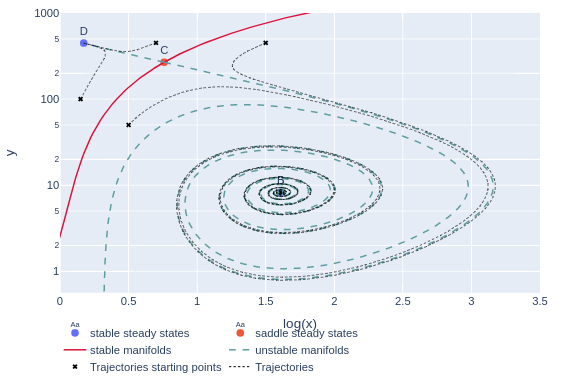
\includegraphics[width=\textwidth]{../figures/fig_phase_portrait_log.png}
         \caption{Portrait de phase (échelle log)}
         \label{fig::phase_portrait_log}
\end{figure}

\begin{figure}[!ht]
    \centering
         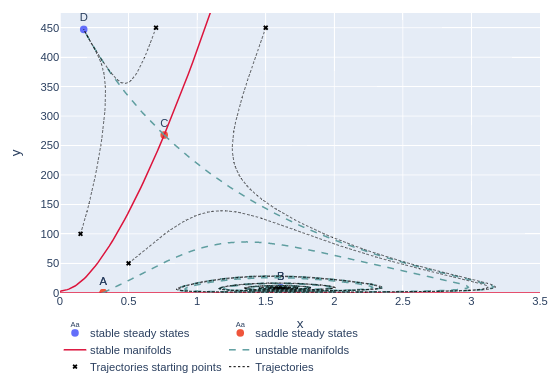
\includegraphics[width=0.9\textwidth]{../figures/fig_phase_portrait.png}
         \caption{Portrait de phase}
         \label{fig::phase_portrait}
\end{figure}



\section{Bifurcations}
On prend $\delta$ comme paramètre de bifurcation. La figure \ref{fig::bifurcations} présente le diagramme de bifurcation.
\begin{figure}[!ht]
    \centering
    
\includegraphics[width=0.75\textwidth]{../figures/fig_bifurcation_legend.png}
    \begin{subfigure}[b]{0.49\textwidth}
         \centering
         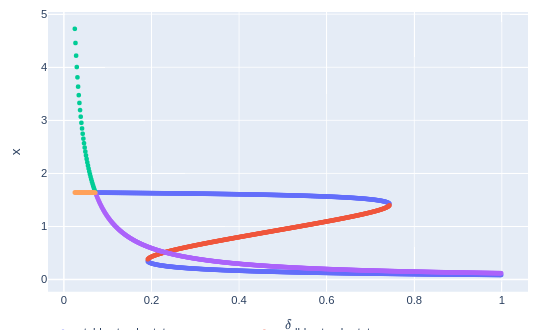
\includegraphics[width=\textwidth]{../figures/fig_bifurcation_x.png}
         \caption{Bifurcations sur $x$}
         \label{fig::bifurcations_x}
     \end{subfigure}
     \hfill
    \begin{subfigure}[b]{0.49\textwidth}
         \centering
         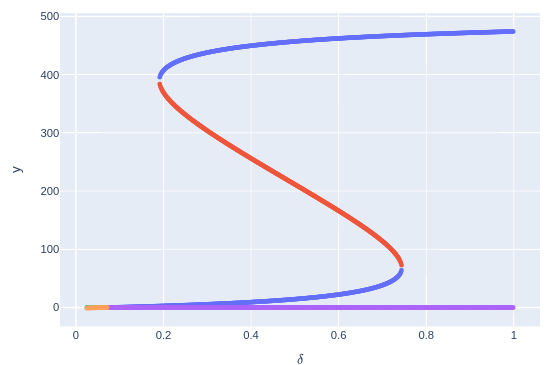
\includegraphics[width=\textwidth]{../figures/fig_bifurcation_y.png}
         \caption{Bifurcations dur $y$}
         \label{fig::bifurcations_y}
     \end{subfigure}
    \caption{Diagramme de bifurcation du modèle avec $\delta$ comme paramètre de bifurcation.}
    \label{fig::bifurcations}
\end{figure}

\paragraph{}
Vers $\delta = 0.07$ on observe une bifurcation transcritique qui échange la stabilité des équilibres A (passe de stable à point-selle) et B (passe de point-selle à stable). 

Vers $\delta = 0.19$ on a une première bifurcation n\oe ud-selle avec apparition des équilibres C (point-selle) et D (stable).

Vers $\delta = 0.74$ on a une deuxième bifurcation n\oe ud-selle avec disparition des équilibres C (point-selle) et B (stable).


\section{Bifurcation hétérocline}
Les bifurcation hétéroclines ont lieu lorsque la variété stable d'un point-selle correspond à la variété instable d'un autre point-selle. La figure \ref{fig::heteroclinic_bifurcation} montre une approximation numérique du phénomène.

\begin{figure}[!ht]
    \centering
    \begin{subfigure}[b]{0.4\textwidth}
         \centering
         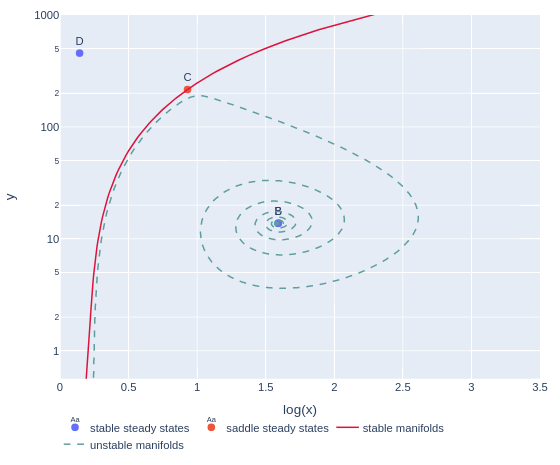
\includegraphics[width=\textwidth]{../figures/fig_heteroclinic_before.png}
         \caption{Portrait de phase avant la bifurcation hétérocline, $\delta = 0.49$}
         \label{fig::heteroclinic_bifurcation_a}
     \end{subfigure}\hfill
     \begin{subfigure}[b]{0.4\textwidth}
         \centering
         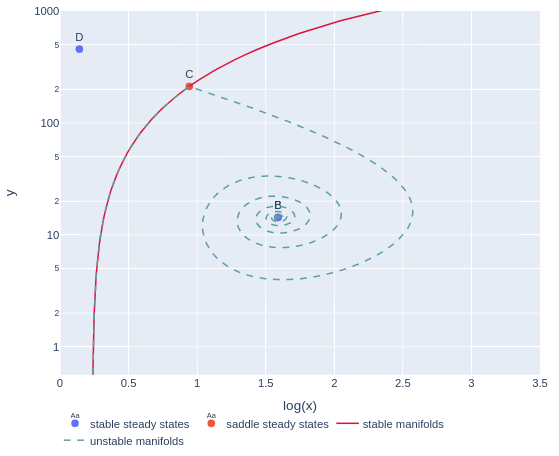
\includegraphics[width=\textwidth]{../figures/fig_heteroclinic.png}
         \caption{Portrait de phase de la bifurcation hétérocline, $\delta = 0.49891$}
         \label{fig::heteroclinic_bifurcation_b}
     \end{subfigure}\\
     \begin{subfigure}[b]{0.4\textwidth}
         \centering
         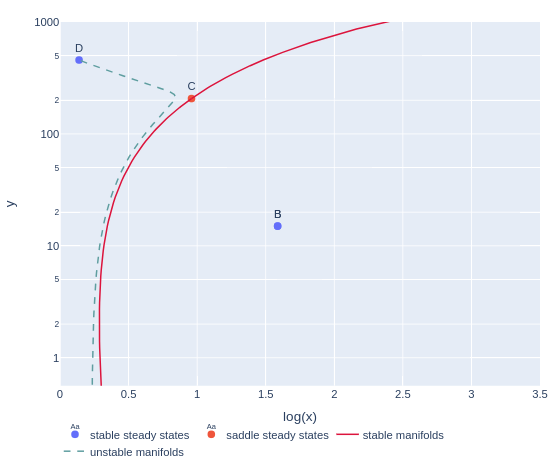
\includegraphics[width=\textwidth]{../figures/fig_heteroclinic_after.png}
         \caption{Portrait de phase après la bifurcation hétérocline, $\delta = 0.51$}
         \label{fig::heteroclinic_bifurcation_c}
     \end{subfigure}
    \caption{Bifurcation hétérocline}
    \label{fig::heteroclinic_bifurcation}
\end{figure}
\paragraph{}
Sur la figure \ref{fig::heteroclinic_bifurcation_a}, avant la bifurcation, on observe qu'une trajectoire partant d'un point du voisinage de A suit la variété instable de A, c'est-à-dire qu'il passe près de C  puis est attiré par l'équilibre stable B.

Sur la figure \ref{fig::heteroclinic_bifurcation_b}, au moment de la bifurcation, les variétés stables et instables de C et de A coïncident. un point du voisinage de A se rapproche donc de C indéfiniment. 

Sur la figure \ref{fig::heteroclinic_bifurcation_c}, après la bifurcation, on observe qu'une trajectoire partant d'un point du voisinage de A passe près de C  puis est attiré par l'équilibre stable D.

\paragraph{} La bifurcation hétérocline a donc échangé le point assymptotiquement attracteur pour les trajectoire partant du voisinage de A. Au moment de la bifurcation, les points du voisinage de A sont assymptotiquement attiré par le point-selle C.

\section{Modèle stochastiques}
Le modèle proposé peut être vu comme une approximation continue d'un processus stochastique discret de naissance-mort. Ce processus stochastique est pertinent dans le cas ou la concentration devient trop faible pour être considérée comme une variable continue. Il n'existe évidemment pas de seuil fixe et définitif mais il est sûr que lorsque le nombre de cellules présentes dans un volume d'intérêt est de l'ordre de la dizaine, l'hypothèse de la concentration continue n'est plus réaliste.

\subsection{\'Ecriture du mod\`ele stochastique}
Les variables du modèle stochastique sont les nombres de cellules effectrices $N_x$ et tumorales ($N_y$) présentes dans un volume donné et non les concentrations de ces cellules. Considérons donc un volume $\Omega$ et réécrivons donc les équations (\ref{equ::modele_adimensionne}) pour $N_x = \Omega x$ et $N_y = \Omega y$: 
\begin{align*}
    &\left\{\begin{aligned}
        \dtau{N_x} &= \Omega \dtau{x} \\
        \dtau{N_y} &= \Omega \dtau{y}
    \end{aligned}\right.\\
    &\left\{\begin{aligned}
        \dtau{N_x} &= \Omega \left(\sigma + \frac{\rho \frac{N_x}{\Omega}\frac{N_y}{\Omega}}{\eta + \frac{N_y}{\Omega}} - \mu \frac{N_x}{\Omega}\frac{N_y}{\Omega} -\delta \frac{N_x}{\Omega}\right) \\
        \dtau{N_y} &= \Omega \left( \alpha \frac{N_y}{\Omega} (1- \beta \frac{N_y}{\Omega}) - \frac{N_x}{\Omega}\frac{N_y}{\Omega}\right)
    \end{aligned}\right.\\
    &\left\{\begin{aligned}
        \dtau{N_x} &= \Omega \sigma + \frac{\rho N_x N_y}{\frac{\eta}{\Omega} + N_y }- \frac{\mu}{\Omega} N_x N_y  -\delta N_x\\
        \dtau{N_y} &= \alpha N_y - \frac{\alpha \beta}{\Omega}N_y^2- \frac{N_x N_y}{\Omega}
    \end{aligned}\right.
\end{align*}\\

Les \'ev\'enements de naissances-morts possibles sont :
\begin{itemize}
\item naissance d'une cellule effectrice:
    \begin{itemize}
        \item par arriv\'ee d'une cellule effectrice avec le taux basal de $\Omega \sigma$
        \item par arriv\'ee de cellules effectrices li\'ee \`a la pr\'esence de cellules tumorales avec un taux $\frac{\rho N_y}{\frac{\eta}{\Omega} + N_y }$
    \end{itemize}
\item mort d'une cellule effectrice :
\begin{itemize}
    \item avec le taux basal de $\delta$
    \item par interaction avec les cellules tumorales au taux $\frac{\mu N_y}{\Omega}$
\end{itemize}
\item naissance d'une cellule tumorale :
\begin{itemize}
    \item au taux constant $\alpha$
\end{itemize}
\item mort d'une cellule tumorale :
\begin{itemize}
    \item li\'e \`a la compétition pour les ressources du milieu au taux $\frac{\alpha \beta}{\omega}N_y$
    \item li\'e \`a l'interaction avec le syst\`eme immunitaire au taux $\frac{N_x}{\Omega}$
\end{itemize}

\subsection{Simulations du mod\`ele stochastique}
\end{itemize}
\section*{Sources}
Les figures présentées ont été produite  à l'aide de la librairie python \texttt{plotly}.\footnote{\url{https://plot.ly/python/}} Le code est disponible en supplément ou à l'adresse \url{https://github.com/celbig/project_popdyn}. Le modèle est implémenté dans le package \texttt{kutznetsov\_model}, le code générant les figures est contenu dans le notebook jupyter \texttt{projet\_pop\_dyn.ipynb}.

\clearpage
\bibliographystyle{plain}
\bibliography{biblio}
\end{document}


